\documentclass[10pt,twocolumn]{article}
\usepackage[margin=0.75in]{geometry}
\usepackage{times}
\usepackage{graphicx}
\usepackage{booktabs}
\usepackage{hyperref}

\title{AI-Powered Misinformation Risk Assistance for Social Media Users}
\author{ENGG1910 Course Project}
\date{}

\begin{document}
\maketitle

\begin{abstract}
We present a misinformation risk assistant for social media users. The system does not make a final true-or-false judgment; instead, it estimates whether a short claim deserves further verification and returns an interpretable risk level. We evaluate the idea on LIAR, a public benchmark of 12.8K political claims labelled by professional fact-checkers. The six LIAR labels are mapped into a binary risk task. Our strongest model combines TF-IDF text features, lightweight metadata features, and logistic regression, reaching 0.743 accuracy, 0.712 F1, and 0.831 ROC-AUC on the official test set. A compact BERT-style transformer fine-tuned under CPU-limited settings reaches 0.609 accuracy and 0.631 ROC-AUC.
\end{abstract}

\section{Introduction}
Social media platforms allow misleading claims to spread before users can verify them. A direct automated truth detector is dangerous because many posts are incomplete, ambiguous, contextual, or developing. We therefore formulate the application as risk assistance rather than truth adjudication.

\section{Task and Data}
We use the LIAR dataset, which contains short political statements collected from PolitiFact with six truthfulness labels. False, barely-true, and pants-fire are assigned to the higher-risk class, while half-true, mostly-true, and true are assigned to the lower-risk class.

\begin{figure}[t]
\centering
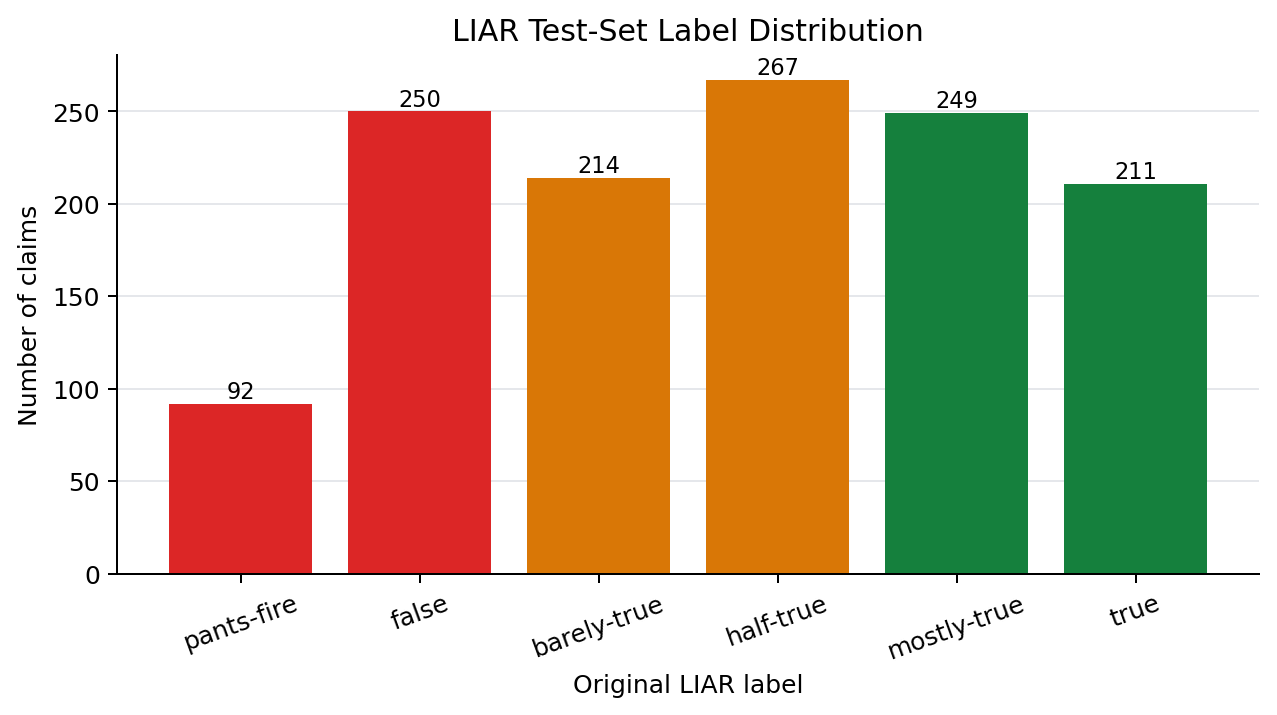
\includegraphics[width=\linewidth]{figures/label_distribution.png}
\caption{Original LIAR label distribution on the official test split.}
\end{figure}

\section{System Architecture}
The application has four stages: input collection, feature extraction, supervised risk scoring, and explanation. The baseline uses TF-IDF unigrams and bigrams plus engineered metadata, while the transformer path tokenizes the claim and fine-tunes a compact BERT classifier.

\section{Models}
The first model is logistic regression over sparse TF-IDF vectors and metadata features. The second model is \texttt{prajjwal1/bert-tiny}, a compact BERT-style transformer fine-tuned for binary classification.

\section{Results}
\begin{table}[t]
\centering
\begin{tabular}{lccccc}
\toprule
Model & Acc. & Prec. & Rec. & F1 & AUC \\
\midrule
TF-IDF + LR & 0.743 & 0.692 & 0.732 & 0.712 & 0.831 \\
BERT-tiny & 0.609 & 0.574 & 0.378 & 0.456 & 0.631 \\
\bottomrule
\end{tabular}
\caption{Test-set comparison between the sparse baseline and compact transformer.}
\end{table}

\begin{figure}[t]
\centering

\includegraphics[width=\linewidth]{figures/model_comparison.png}
\caption{Model comparison across five classification metrics.}
\end{figure}

\begin{figure}[t]
\centering

\includegraphics[width=\linewidth]{figures/roc_curves.png}
\caption{ROC curves for the baseline and compact transformer.}
\end{figure}

\section{Analysis}
The TF-IDF logistic regression model performs best, with 0.743 accuracy, 0.712 F1, and 0.831 ROC-AUC. The compact transformer is weaker under our limited compute setting, indicating that model complexity alone is not sufficient.

\begin{figure}[t]
\centering

\includegraphics[width=\linewidth]{figures/risk_distribution.png}
\caption{Predicted risk-level distribution from the baseline assistant.}
\end{figure}

\begin{figure}[t]
\centering

\includegraphics[width=\linewidth]{figures/baseline_confusion_matrix.png}
\caption{Confusion matrix for TF-IDF logistic regression.}
\end{figure}

\begin{figure}[t]
\centering

\includegraphics[width=\linewidth]{figures/transformer_confusion_matrix.png}
\caption{Confusion matrix for the compact transformer.}
\end{figure}

\section{Ethical Considerations}
The system should not be used as an automatic censorship tool. False positives may unfairly reduce trust in legitimate speech, while false negatives may give users false confidence. A deployed system should minimize private account and repost data collection.

\section{Conclusion}
We built a reproducible misinformation risk assistant using LIAR. The project demonstrates that effective AI applications require careful task framing, data preparation, explanation, and ethical boundaries, not only powerful models.

\section*{References}
Wang, W. Y. 2017. Liar, Liar Pants on Fire: A New Benchmark Dataset for Fake News Detection. ACL.

Devlin, J., Chang, M.-W., Lee, K., and Toutanova, K. 2019. BERT: Pre-training of Deep Bidirectional Transformers for Language Understanding. NAACL.

\end{document}
